\chapter{高次元エクスパンダー概論}
高次元エクスパンダーとはグラフのエクスパンダー性を単体複体に拡張した概念であり,
具体的には単体複体の面上で定義されたある種のランダムウォークが速く混交するという性質を意味する.
本チャプターでは高次元エクスパンダーの概要と重要な性質を紹介し,
次のチャプターにおいて具体的な応用として近年解決されたマトロイドに関する重要な未解決問題Micali--Vazirani予想の証明を与える.

\section{定義}
まずは単体複体に関する基礎的な用語を定義していく.
文脈によっては単体複体は多面体などを貼り合わせた幾何的な概念を指すこともあるが,
本講義では組合せ的ないわゆるset system (ハイパーグラフ) としての単体複体を扱う.

\begin{definition}{単体複体}{simplicial complex}
有限集合$V$と$V$の部分集合族$\F\subseteq 2^V$であって部分集合で閉じているもの(すなわち, $\sigma\subseteq \tau \in \F \Rightarrow \sigma\in \F$)の組$X=(V,\F)$を\emph{単体複体 (simplicial complex)}という.
集合族$\F$の元を\emph{面 (face)}と呼び,
面$\sigma \in \F$の\emph{次元 (dimension)}を$\dim \sigma = \abs{\sigma} - 1$とする\footnote{特に, 空集合$\emptyset \in \F$の次元は$-1$である.}.
単体複体$X$の次元を$\dim X = \max\cbra{\dim \sigma \colon \sigma \in \F}$とする.

次元$d$の単体複体$X$は(包含関係に関して)極大な面の次元が全て$d$に等しいとき, \emph{純粋 (pure)}であるという.
整数$-1 \le k \le \dim X$に対し$X(k) = \cbra*{\sigma \in \F\colon \dim \sigma = k }$とする.
特に断りのない限り, $X(0)=V$を仮定する
(そうでなければ$V$として$V=X(0)$とした単体複体を考える).
\end{definition}
面の次元の概念は単体複体の幾何的な表現に由来する.
このイメージになぞらえて,
次元$0$の面を\emph{頂点 (vertex)}, 次元$1$の面を\emph{辺 (edge)}と呼ぶことがある.
次元$2$以上の任意の単体複体$X$に対して$(X(0),X(1))$はグラフである.

\paragraph*{例1.}
グラフ$G=(V,E)$に対し, 空集合, $V$, $E$からなる部分集合族
$\F = \{\emptyset\} \cup \cbra*{\{v\}\colon v \in V} \cup E$考えると,
$(V,\F)$は単体複体である.

\paragraph*{例2.}
有限集合$V$に対し,
$\F = \binom{V}{\le k} \defeq \cbra*{ \sigma \subseteq V \colon |\sigma|\le k}$としたとき, $(V,\mathcal{F})$は純粋な$(k+1)$-次元の単体複体である.

\paragraph*{例3.}
閉路を含まないグラフを\emph{森 (forest)}といい, 連結な森を\emph{木 (tree)}という.
連結グラフ$G$の部分グラフであって木であるものを\emph{全域木 (spanning tree)}という (cf. \cref{def:graph}).
グラフ$G=(V,E)$に対し,
森であるような部分グラフの辺集合からなる集合族$\F\subseteq 2^E$は単体複体である.
すなわち,
\begin{align*}
    \F = \cbra*{ F \subseteq E \colon \text{部分グラフ$(V,F)$は森}}
\end{align*}
に対して$(E,\F)$は単体複体である.
簡単のため$G$を連結グラフであるとすると, $(E,\F)$の極大面は$G$の全域木に対応し, その次元は$n-2$に等しい.
すなわち$(E,\F)$は純粋な$(n-2)$-次元単体複体である.

なお, グラフ$G$が連結でない場合, 異なる連結成分に属する二頂点$u,v$を縮約し一つの頂点として扱うことによって$(V,\F)$の構造を変えないまま連結成分数を減らすことができるので, 連結性を仮定しても一般性を失わない.

\paragraph*{例4.}
実行列$A\in \Real^{n\times m}$ (ただし$m\ge n$) の行ベクトルを$\vec{a}_1,\dots,\vec{a}_n$とする.
集合$V=\{1,\dots,n\}$の部分集合族であって, 線形独立な行ベクトル集合のインデックスとなるものの全体を$\F$とする.
すなわち
\[
    \F = \cbra*{ I \subseteq V\colon (\vec{a}_i)_{i\in I}\text{は線形独立}}
\]
とすると, $(V,\F)$は純粋な単体複体であり, その次元は$A$のランク$\mathrm{rank}(A)$に対し$\mathrm{rank}(A)-1$となる.

\paragraph*{例5.}
部集合$L,R$を持つ二部グラフ$G=(V,E)$を考える.
辺部分集合$M\subseteq E$は, 部分グラフ$(V,M)$の全ての頂点の次数が高々$1$であるとき\emph{マッチング (matching)}という.
マッチング$M$の部分集合$M'\subseteq M$もまたマッチングであるため,
グラフ$G$のマッチング全体からなる辺部分集合族$\F\subseteq 2^E$に対し, $(E,\F)$は単体複体である.
一般に極大マッチングのサイズは異なる場合があるのでこの単体複体は純粋ではない (\cref{fig:matching}).
\begin{figure}[htbp]
    \begin{center}
        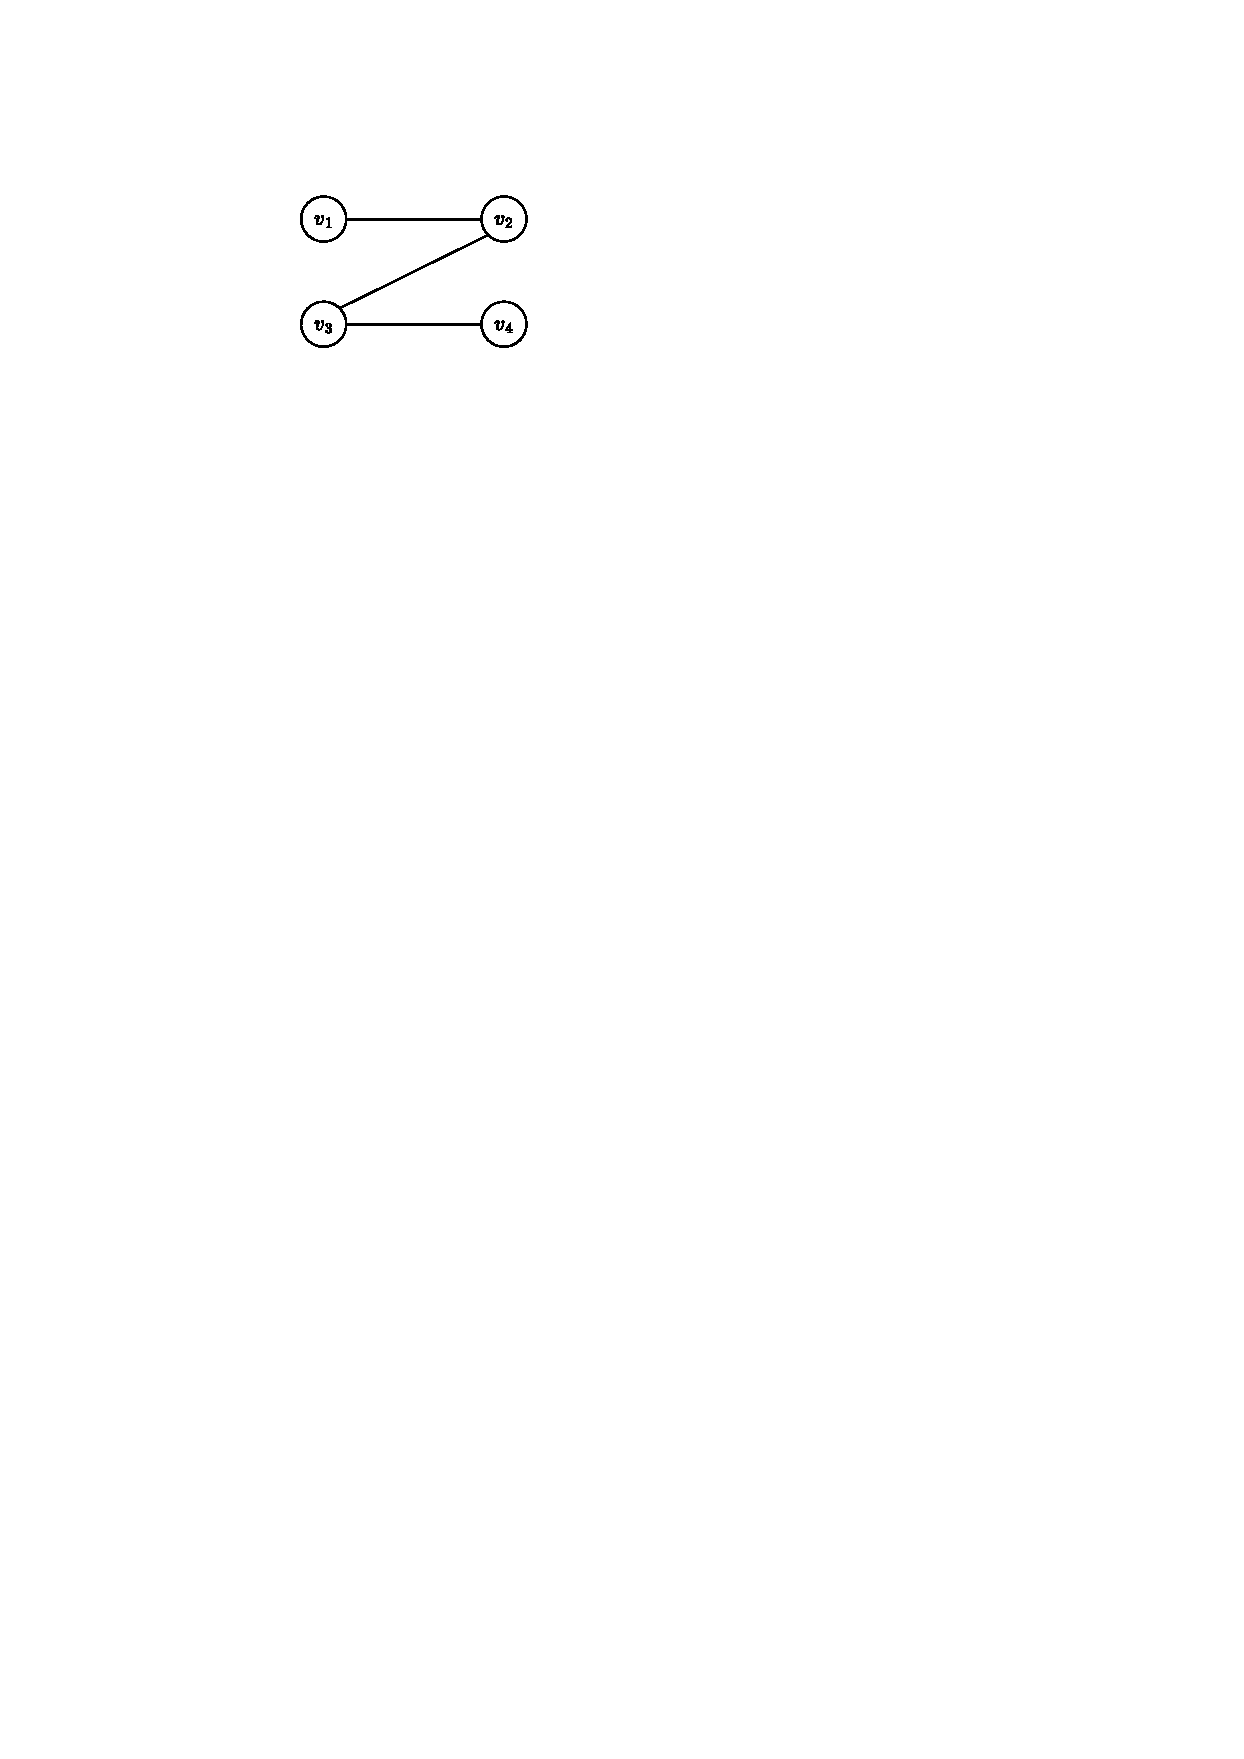
\includegraphics[width=5cm]{images/matching.pdf}
    \end{center}
    \caption{マッチング$M_1=\{v_1,v_2\},\{v_3,v_4\}\}$と$M_2=\{\{v_2,v_3\}\}$はどちらも極大である. \label{fig:matching}}
\end{figure}

\paragraph*{例6.}
グラフ$G=(V,E)$の頂点部分集合$U\subseteq V$は, $U$に属する任意の二頂点間に辺がある(すなわち$\binom{U}{2}\subseteq E$)とき, \emph{クリーク (clique)}\footnote{cliqueとは派閥を意味する英単語である.}という.
特に, 単一頂点からなる集合$\{u\}$や$\emptyset$もクリークである.
クリークの部分集合もまたクリークなので,
グラフ$G$の全てのクリークからなる頂点集合族を$\F$とすると, $(V,\F)$は単体複体である.

\begin{definition}{リンクとスケルトン}{link and skelton}
    単体複体$X=(V,\F)$を考える.
    面$\sigma \in \F$の\emph{リンク (link)}とは単体複体$(V\setminus \sigma, \F_{\sigma})$であって集合族$\F_\sigma$が
    \[
        \F_\sigma = \cbra*{ \tau \setminus \sigma \colon \sigma \subseteq \tau \in \F }
    \]
    で与えられるものである.
    次元$k$以下の面の集合
    \[
        \F_k = \cbra*{ \sigma \in \F \colon \dim \sigma \le k}
    \]
    に対し$(V,\F_k)$を\emph{$k$-スケルトン ($k$-skelton)}という.
\end{definition}
面$\sigma$のリンクとは, $\sigma$を「縮約」して得られる単体複体である.

%\end{definition}


\section{単体複体上の三つのランダムウォーク}
グラフ上のランダムウォークは頂点集合上で遷移するものを考えていたが,
単体グラフ上のランダムウォークは異なる次元の面の間で遷移するものを考える.
具体的には, \cref{sec:graph up and down walk}で考えたようにある次元$i$の面から次元$i+1$の面に遷移する上昇ウォークと逆に次元$i+1$の面から次元$i$の面に遷移する下降ウォークである.
上昇ウォークと下降ウォークが互いに随伴の関係になるようにするため, 各$X(i)$上での定常分布も定義する.
また, 各リンクの$2$-スケルトン上のランダムウォークも考える.
この「局所的な」ランダムウォークと$X(k)$上の二種類のランダムウォークの関係性がグラフ上のランダムウォークとの一番重要な差分となる.

\subsection{下降ウォークと定常分布}
まず, \cref{sec:graph up and down walk}で考えた下降ウォークを単体複体に拡張し, $X(d-1)$上では一様分布を定常分布とすることによって帰納的に各$X(i)$上での定常分布を定める.
\begin{definition}{下降ウォークと面上の定常分布}{down walk and stationary distribution}
    純粋な$d$次単体複体$X=(V,\F)$を考える.
    各$i=0,\dots,d-1$に対し
        確率行列$\Pdown_i \in [0,1]^{X(i) \times X(i-1)}$を
        \[
            \Pdown_i(\tau,\sigma) = \begin{cases}
                \frac{1}{i+1}	& \tif \sigma \subseteq \tau,\\
                0 & \totherwise
            \end{cases}
        \]
        とする.
    各$i=0,\dots,d-1$に対して, $X(i)$上の分布$\pi_i \in [0,1]^{X(i)}$を
        \begin{itemize}
        \item $i=d-1$のとき, $\pi_{d-1}$は$X(d-1)$上の一様分布. すなわち$\pi_{d-1}(\sigma) = \frac{1}{\abs{X(d-1)}}$
        \item $\pi_{i+1}$が定義されているとき, $\pi_i = \pi_{i+1}\Pdown_{i+1}$
        \end{itemize}
    で定める.
    分布$\pi_i$を($i$次の)定常分布と呼ぶ.
\end{definition}
面$\tau \in X(i+1)$に対して$\Pdown_{i+1}(\tau,\cdot)$で定まる$X(i)$上の分布は, 面$\tau$に含まれる頂点$u$を一様ランダムに選んだときの$\sigma = \tau \setminus\{u\}$の分布と等しい.
この分布は, まず一様ランダムに$X(d)$から面を選び, その中から一様ランダムに選ばれた$i+1$個の頂点からなる$X(i)$の面のなす分布である.
特に全ての$\sigma\in X(i)$に対し$\pi_i(\sigma)=0$である
(そうでなければ, $\pi_d$が一様分布であることに反する).
ある面$\tau\in X(i+1)$から分布$\Pdown_{i+1}(\tau,\cdot)$に従ってランダムに選ばれた面$\sigma$に遷移する過程を\emph{下降ウォーク (down walk)}と呼ぶ.

\subsection{上昇ウォーク}
\cref{def:down walk and stationary distribution}では次元$i$の面から次元$i-1$に遷移する下降ウォークを与えた.
同様に, 次元$i$の面から次元$i+1$の面に遷移する上昇ウォークを, $X(i)$と$X(i+1)$の間の詳細釣り合い条件が成り立つように定義する.
%
\begin{definition}{上昇ウォーク}{up walk}
    純粋な$d$次単体複体$X=(V,\F)$を考える.
    各$i=-1,\dots,d-2$に対し
        確率行列$\Pup_i \in [0,1]^{X(i) \times X(i+1)}$を
    \begin{align*}
        \Pup_i(\sigma,\tau) &= \frac{\pi_{i+1}(\tau)}{\pi_i(\sigma)}\Pdown_{i+1}(\tau,\sigma) \\
        &= \begin{cases}
            \frac{\pi_{i+1}(\tau)}{(i+1)\pi_i(\sigma)}	& \tif \sigma\subseteq \tau,\\
            0 & \totherwise
        \end{cases}
    \end{align*}
    で定める.
\end{definition}
%
二つの面集合$X(i)$と$X(i+1)$を部集合とする二部グラフを考えればわかりやすい.
それぞれの部集合には$\pi_i,\pi_{i+1}$が定常分布として付随しており,
上昇ウォーク$\Pup_i$と下降ウォーク$\Pdown_{i+1}$は詳細釣り合い条件
\[
    \forall \sigma\in X(i),\tau\in X(i+1),\,\pi_i(\sigma)\Pup_i(\sigma,\tau) = \pi_{i+1}(\tau)\Pdown_{i+1}(\tau,\sigma)
\]
を満たしている.

なお, 下降ウォーク$\Pdown_{i}$と上昇ウォーク$\Pup_i$の添字$i$は遷移の開始地点の面の次元としている.
%
\begin{remark}{「上昇」「下降」の名称}{up and down}
    非常にややこしいのだが,
    上昇ウォークと下降ウォークをそれぞれランダムウォークの遷移確率行列とみなすか左から作用させる作用素としてみなすかによって「上昇」「下降」の意味合いが反転してしまう.
    確率行列としての上昇ウォークは$\Pup_i \in [0,1]^{X(i)\times X(i+1)}$で表せる.
    これを左から作用させる作用素とみなすと
    $\Pup_i\colon \Real^{X(i+1)} \to \Real^{X(i)}$
    であるので, 次元を一つ落とすように見えてしまうのである.
    下降ウォークについても同様である.
    本講義はランダムウォークを主眼におき, 右から作用させるときの$\Pup_i,\Pdown_i$に興味があるので\cref{def:down walk and stationary distribution}, \ref{def:up walk}の呼称を採用している.
    なお, 通常の可逆なランダムウォーク(\cref{def:reversible})は内積$\piprod{\cdot,\cdot}$の意味で左右どちらから作用させても本質的に同じであるのでこのような煩雑な話は怒らない.
\end{remark}
\begin{remark}{随伴}{HDX adjoint}
    各$X(i)$に対して空間$\ell^2_{\pi_i}(X(i))$, 
    すなわち, \cref{def:naiseki}と同様にして$\Real^{X(i)}$に内積$\abra{\cdot,\cdot}_{\pi_i}$が導入された空間を定義できる.
    このとき, 
    \[\Pup_i\colon \ell^2_{\pi_{i+1}}(X(i+1)) \to \ell^2_{\pi_{i}}(X(i))\]
    と
    \[\Pdown_{i+1}\colon \ell^2_{\pi_{i}}(X(i)) \to \ell^2_{\pi_{i+1}}(X(i+1))\]
    は互いに随伴の関係にある.
    すなわち, 任意の$f\in \ell^2_{\pi_i}(X(i)),g\in \ell^2_{\pi_{i+1}}(X(i+1))$に対して
    \begin{align} \abra{\Pup_i f, g}_{\pi_{i+1}} = \abra{ f,\Pdown_{i+1}g }_{\pi_i} \label{eq:adjoint up and walk}\end{align}
    が成り立つ.
\end{remark}
%
\begin{exercise}{}{adjoint check}
    \cref{eq:adjoint up and walk}を確認せよ.
    すなわち, \cref{def:down walk and stationary distribution}で定義された定常分布$\pi_i,\pi_{i+1}$および任意の二つの関数$f\colon X(i) \to \Real,g\colon X(i+1) \to \Real$に対して
    \[ \sum_{\sigma \in X(i)} \pi_i(\sigma) f(u) = \sum_{\tau \in X(i+1)} \pi_{i+1}(\tau) g(\tau) \]
を確認せよ.
\end{exercise}

\subsection{局所的なランダムウォーク}
全てのリンクの$2$-スケルトン上での局所的な重み付きランダムウォークを考える.
重み付きランダムウォークについては\cref{def:weighted random walk}を参照されたい.
%
\begin{definition}{局所ランダムウォーク}{local random walk}
    純粋な$d$次元単体複体$X = (V,\F)$を考える.
    次元$i \le d-2$の面$\sigma \in \F$に対し,
        リンク$X_\sigma$の$2$-スケルトンを$G_\sigma = (V_\sigma,E_\sigma)$とする.
    このグラフの辺重み$w_\sigma\colon E_\sigma \to [0,1]$を
    \[ w_\sigma(e) = \pi_i(\sigma\cup e) \]
    で定め, これによって定まる$V_\sigma$上の重み付きランダムウォークを面$\sigma$に関する\emph{局所ランダムウォーク (local random walk)}と呼び\footnote{このランダムウォークの概念は高次元エクスパンダーの文脈ではほぼ必ず登場するが, 特に標準的な用語が与えられてはいないので、「局所ランダムウォーク」という用語は本講義だけの局所的なものとする.}, 遷移確率行列を$P_\sigma\in [0,1]^{V_\sigma\times V_\sigma}$とする.
\end{definition}
%
必ずしも局所ランダムウォークが既約性や非周期性を持つとは限らない(すなわち, グラフ$G_\sigma$が非連結だったり二部グラフになりうる)が,
可逆性は必ず満たすことに注意せよ.
%
\section{高次元エクスパンダーの目的}
そもそも単体複体上のランダムウォークを考えて何が嬉しいのだろうか?

%
\section{局所エクスパンダー}
純粋な単体複体のエクスパンダー性を定義する.
任意の面$\sigma$に対し$G_\sigma$上での局所ランダムウォークの第二固有値が小さいとき, その単体複体は局所的エクスパンダー性をもつという.
\begin{definition}{局所エクスパンダー性}{local expander}
    純粋な$d$次元単体複体$X=(V,\F)$は,
    任意の面$\sigma\in\F$に対し$\lambda_2(P)\le \lambda$を満たすとき,
    \emph{局所$\lambda$-エクスパンダー (local $\lambda$-expander)}であるという.
    より一般に, 任意の$i=-1,\dots,d-2$と任意の面$\sigma\in X(i)$に対して$\lambda_2(P_\sigma) \le \lambda_i$を満たすとき, 単体複体$X$は局所$(\lambda_{-1},\dots,\lambda_{d-2})$-エクスパンダーであるという.
\end{definition}
%
\begin{remark}{}{HDX term}
    単体複体のエクスパンダー性は比較的新しい分野であり, その理論的整備が十分でないゆえに, 同じ概念であってもそれぞれの論文によって異なる用語で呼ばれている.
    例えば局所$\lambda$-エクスパンダーという用語は
    \begin{itemize}
    \item $\lambda$-HDX
    \item local spectral $\lambda$-expander
    \end{itemize}
    などと呼ばれている.
    本講義で扱う用語はランダムウォークにおける応用を念頭におきつつ,
    エクスパンダーグラフの用語との整合性を総合的に判断して訳している (例えば局所$\lambda$-\emph{スペクトル}エクスパンダーと呼ぶと\cref{def:expander}においてエクスパンダーグラフを\emph{スペクトル}エクスパンダーと呼ぶべきであろうことから「スペクトル」の形容詞を省いた).
\end{remark}


\section{Oppenheimのトリクルダウン定理}

\section{高次元エクスパンダーの応用}
理論計算機科学における高次元エクスパンダーの応用を簡単にまとめる.
特にマトロイドに関するものは次チャプターにて解説する.